\begin{blocksection}
\question What would Java display? Draw a box-and-pointer diagram to find out!

\begin{lstlisting}
public class Horse {
    Horse same;
    String jimmy;
    public Horse(String lee) {
        jimmy = lee;
    }
    public Horse same(Horse horse) {
        if (same != null) {
            Horse same = horse;
            same.same = horse;
            same = horse.same;
        }
        return same.same;
    }
    public static void main(String[] args) {
        Horse horse = new Horse("you've been");
        Horse cult = new Horse("horsed");
        cult.same = cult;
        cult = cult.same(horse);
        System.out.println(cult.jimmy);
        System.out.println(horse.jimmy);
    }
}
\end{lstlisting}

\begin{solution}[1.5in]
\begin{verbatim}
horsed
you've been
\end{verbatim}

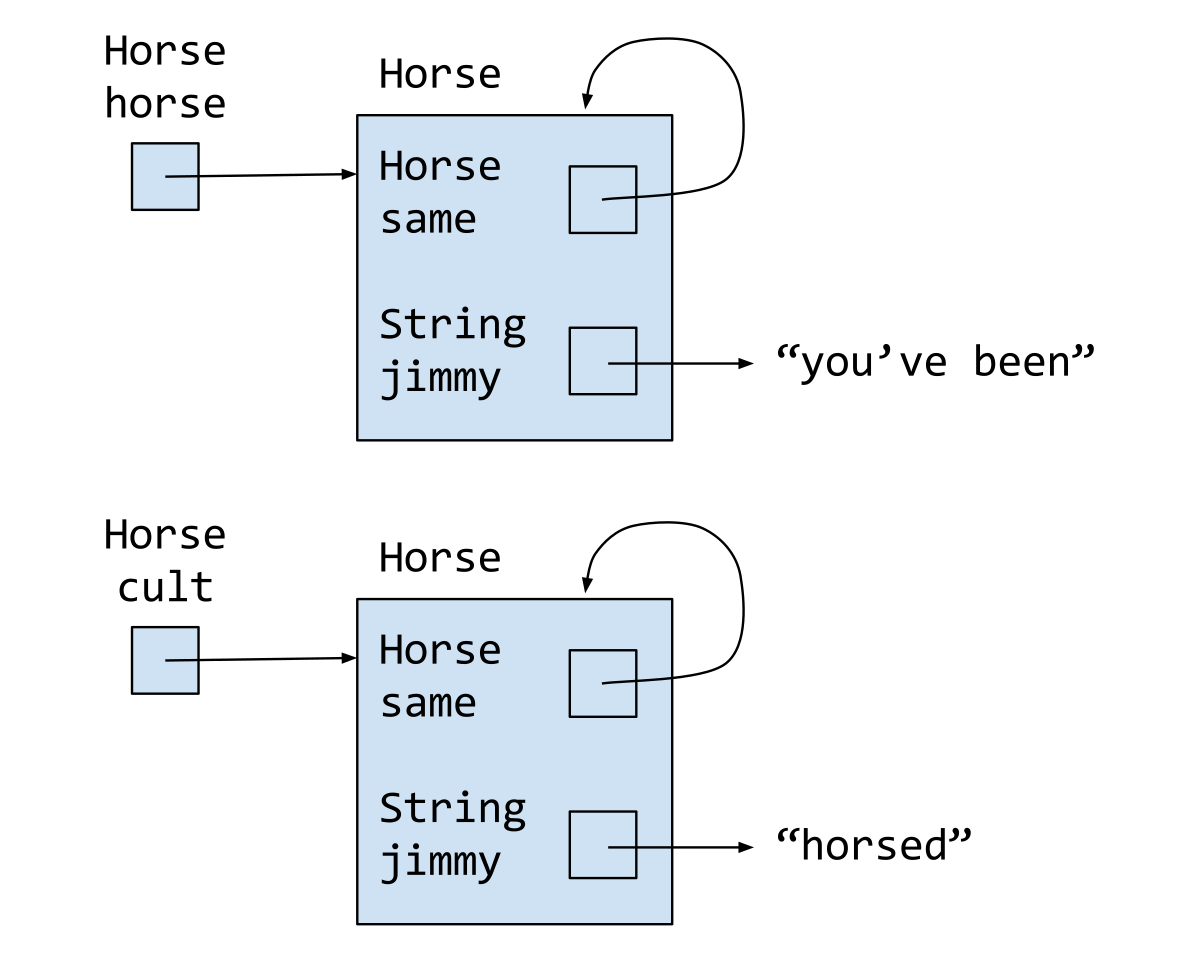
\includegraphics[height=1.7in]{samehorse}

\textbf{Meta:} One good way to teach this question is by drawing out an
environment diagram, and very carefully figuring out what needs to be assigned
to what. The purpose of the question is to realize that Java will first look
inside the local scope to find a variable and then in the instance/class scope.
\end{solution}
\end{blocksection}
